%%%%%% CMB-S4 Lensing Chapter  %%%%%%%%%%%%%%%%
 
\chapter{CMB Lensing}
%\renewcommand*\thesection{\arabic{section}}

\begin{center}
{\small \it (send feedback on this chapter to \href{mailto:s4_lensing@cosmo.uchicago.edu}{s4\_lensing@cosmo.uchicago.edu})}
\end{center}



\def\nnu{N_{\mathrm eff}}
\def\gtrsim{\raise-.75ex\hbox{$\buildrel>\over\sim$}}
%\definecolor{orange}{rgb}{1,0.3,0}
%\newcommand\comments[1]{\textcolor{orange}{[#1]} }
%%%%%%%%%%%%%%%%%%%%%%%%%%%%%%%%%%%%%%%%%%%%%%%%%%%%%%%%%%
%%%%%%%%%%%%%%%%%%%%%%%%%%%%%%%%%%%%%%%%%%%%%%%%%%%%%%%%%%
%%%%%%%%%%%%%%%%%%%%%%%%%%%%%%%%%%%%%%%%%%%%%%%%%%%%%%%%%%
%%%%%%%%%%%%%%%%%%%%%%%%%%%%%%%%%%%%%%%%%%%%%%%%%%%%%%%%%%

\section{Introduction to CMB Lensing}
\label{sec:lensing_intro}

As CMB photons travel from the last scattering surface to Earth, their travel paths are bent by interactions with intervening matter in a process known as \textit{gravitational lensing}.
This process distorts the observed pattern of CMB anisotropies, which has two important consequences:\\
 
$\bullet$ CMB lensing encodes a wealth of statistical information about the entire large-scale structure (LSS) mass distribution, which is sensitive to the properties of neutrinos and dark energy.\\

$\bullet$ CMB lensing distortions obscure our view of the primordial Universe, limiting our power to constrain inflationary signals; removing this lensing noise more cleanly brings the early Universe and any inflationary signatures into sharper focus.\\


Gravitational lensing of the CMB can be measured by relying on the fact that the statistical properties of the primordial CMB are well known.
The primordial (un-lensed) CMB anisotropies are statistically isotropic.
Gravitational lensing shifts the apparent arrival direction of CMB photons, which breaks the primordial statistical isotropy;
lensing thus correlates previously independent Fourier modes of the CMB temperature and polarization fields.
These correlations can be used to make maps of the LSS projected along the line-of-sight; see the discussion in Section \ref{kappaMap}.

A CMB-S4 experiment will make radical improvements in CMB lensing science:
high sensitivity will enable lensing maps that have much higher signal to
noise; the high polarization sensitivity will allow
lensing maps that are much less sensitive to foreground contamination;
multi-frequency coverage will greatly reduce foreground 
contamination in the temperature-based lensing estimates, 
allowing lensing maps with higher resolution; and
large area coverage will provide maps for cross-correlation with maps of large
scale structure from next generation surveys, including WFIRST, Euclid, and LSST.


The information contained in lensing mass maps can be accessed and used in several ways.
First, the power spectrum of the lensing deflection map is sensitive to any physics that modifies how structure grows, such as dark energy, modified gravity, and the masses of neutrinos.
In Section \ref{measuringLensing}, we discuss how the lensing power spectrum is measured.
Second, lensing mass maps can be compared to other tracers of LSS at lower redshifts such as the distribution of galaxies and optical weak lensing shear maps.  By cross correlating, for example, CMB lensing and optical shear mass maps, which are each derived from lensed sources at widely differing redshifts, one can enhance dark energy constraints and improve the calibration of systematic effects.
Cross-correlation science with CMB lensing maps is discussed in Section \ref{cross}.
Finally, lensing distortions partially obscure potential signatures of cosmic inflation in the primordial B-mode polarization signal.
With precise measurements, this lensing-induced noise can be characterized and removed in a procedure known as ``delensing.''
Because B-mode polarization measurements from CMB-S4 are expected to be lensing-noise dominated, delensing will be critical to maximize the information we can infer about cosmic inflation; see the discussion in Section \ref{delens}.

We discuss systematics from astrophysical and instrumental effects that can impact the lensing signal as well as ways to mitigate them in Section \ref{syst}.  Section \ref{forecasts} discusses forecasted parameter constraints with and without CMB lensing and demonstrates the importance of CMB lensing measurements for all the key CMB-S4 science goals.  


%%%%%%%%%%%%%%%%%%%%%%%%%%%%%%%%%%%%%%%%%%%%%%%%%%%%%%%%%%%
\section{Measuring CMB Lensing}\label{measuringLensing}

\subsection{Constructing a Lensing Map}\label{kappaMap}

A map of the CMB lensing deflection field is a direct probe of the projected matter distribution that exists in the observable Universe. This lensing map is a fundamental object for nearly all areas of CMB lensing science: it is used to measure the lensing power spectrum, measure cross correlations between CMB lensing and external data sets, and to delens maps of the B-mode polarization.  


\begin{figure}[htbp]
\centering
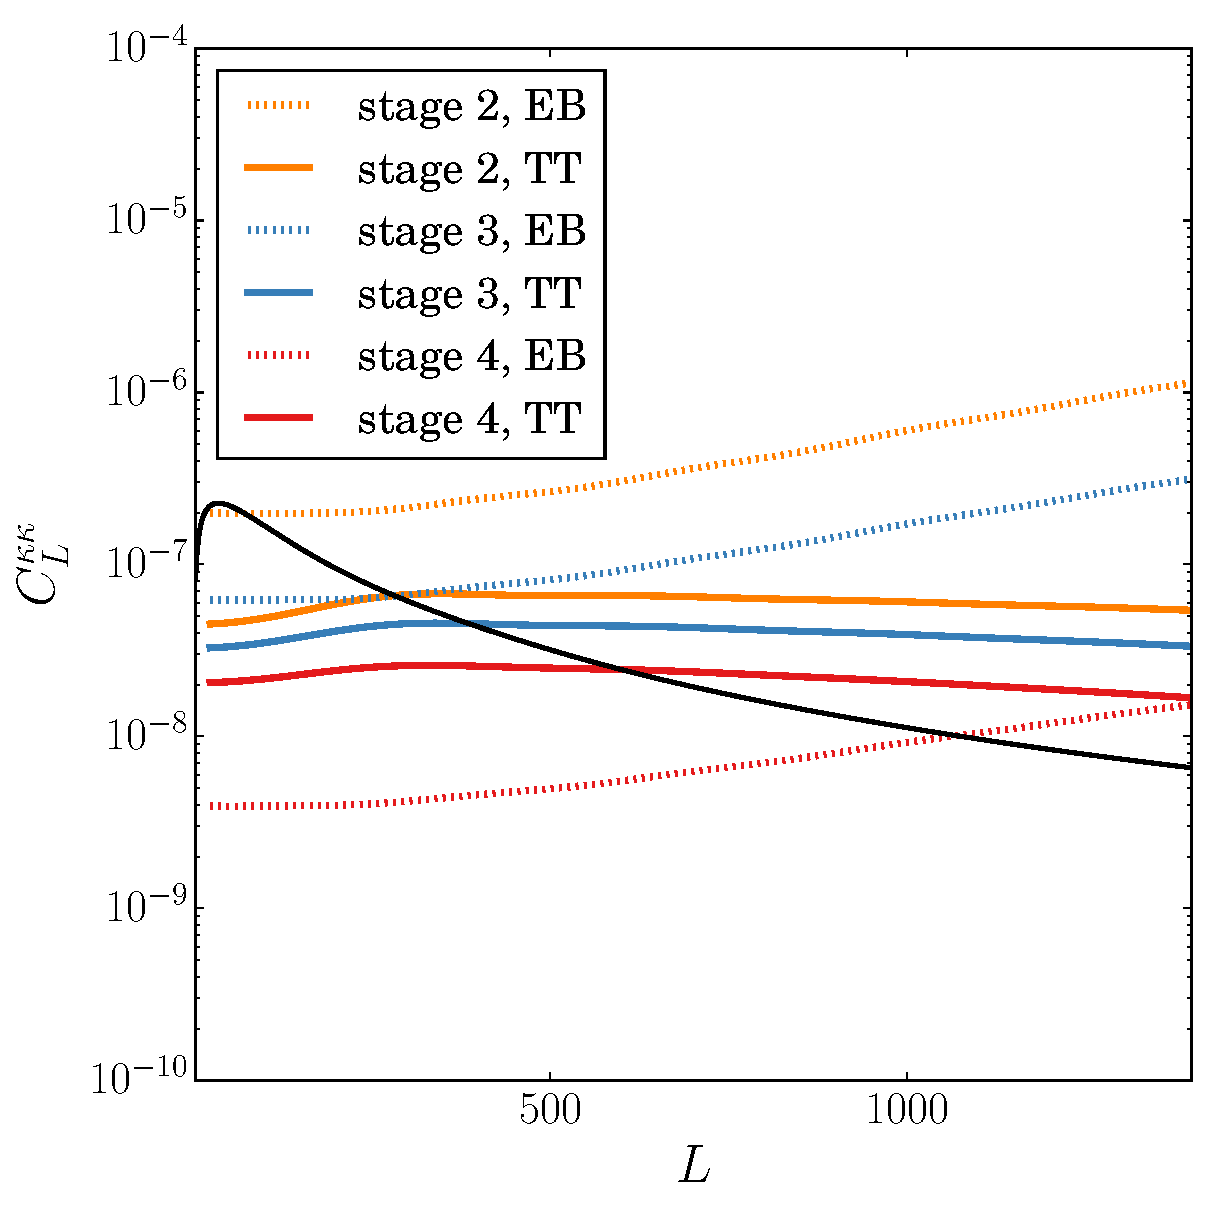
\includegraphics[width=0.5\textwidth]{CMBLensing/n0s_s4.pdf}
\caption{Signal and noise-per-mode curves for three experiments. ``Stage 2'' is meant to represent a current-generation survey like SPTpol or ACTPol and has $\Delta_T = 9 \mu$K-arcmin; ``Stage 3'' is an imminent survey like SPT-3G or AdvACT, with $\Delta_T = 5 \mu$K-arcmin; and ``Stage 4'' has a nominal noise level of  $\Delta_T = 1 \mu$K-arcmin.   These noise-per-mode curves do not depend on the area of sky surveyed.  All experiments assume a 1.4' beam.}  
\label{n0s_s4}
\end{figure}


To date, all maps of the lensing field have been constructed using the quadratic estimator by \cite{Hu:2001kj}.  This estimator uses information about the off-diagonal mode-coupling in spherical harmonic space that lensing induces in order to reconstruct the deflection field.  An estimate for the amount of lensing on a given scale is obtained by averaging over pairs of CMB modes in harmonic space separated by this scale. CMB-S4 will greatly improve over existing measurements by having high angular resolution and high sensitivity for both temperature and polarization CMB maps.

One way that the high angular resolution and sensitivity
of CMB-S4 improves upon the Planck measurement is simply
by increasing the number of CMB modes imaged on scales smaller than the Planck beam.  Imaging CMB modes between $l=2000$ and 4000, which can be achieved with CMB-S4 yields considerable gain in the accuracy of the lensing power spectrum measurement.

\begin{figure}[htbp]
\centering
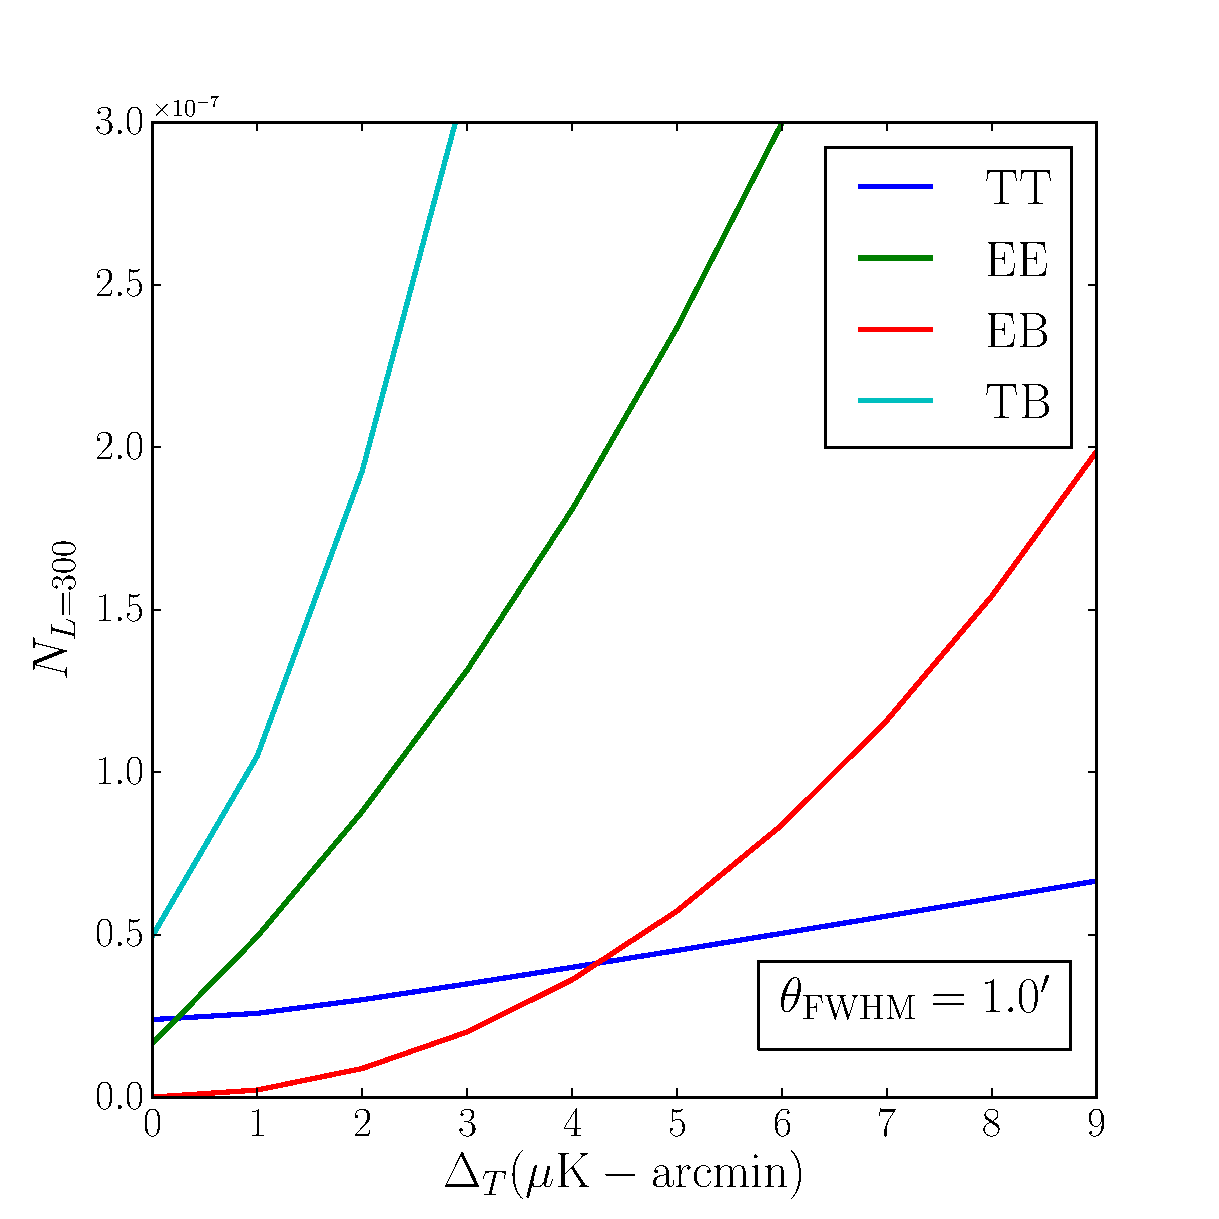
\includegraphics[width=0.45\textwidth]{CMBLensing/ell300_1_00.pdf}
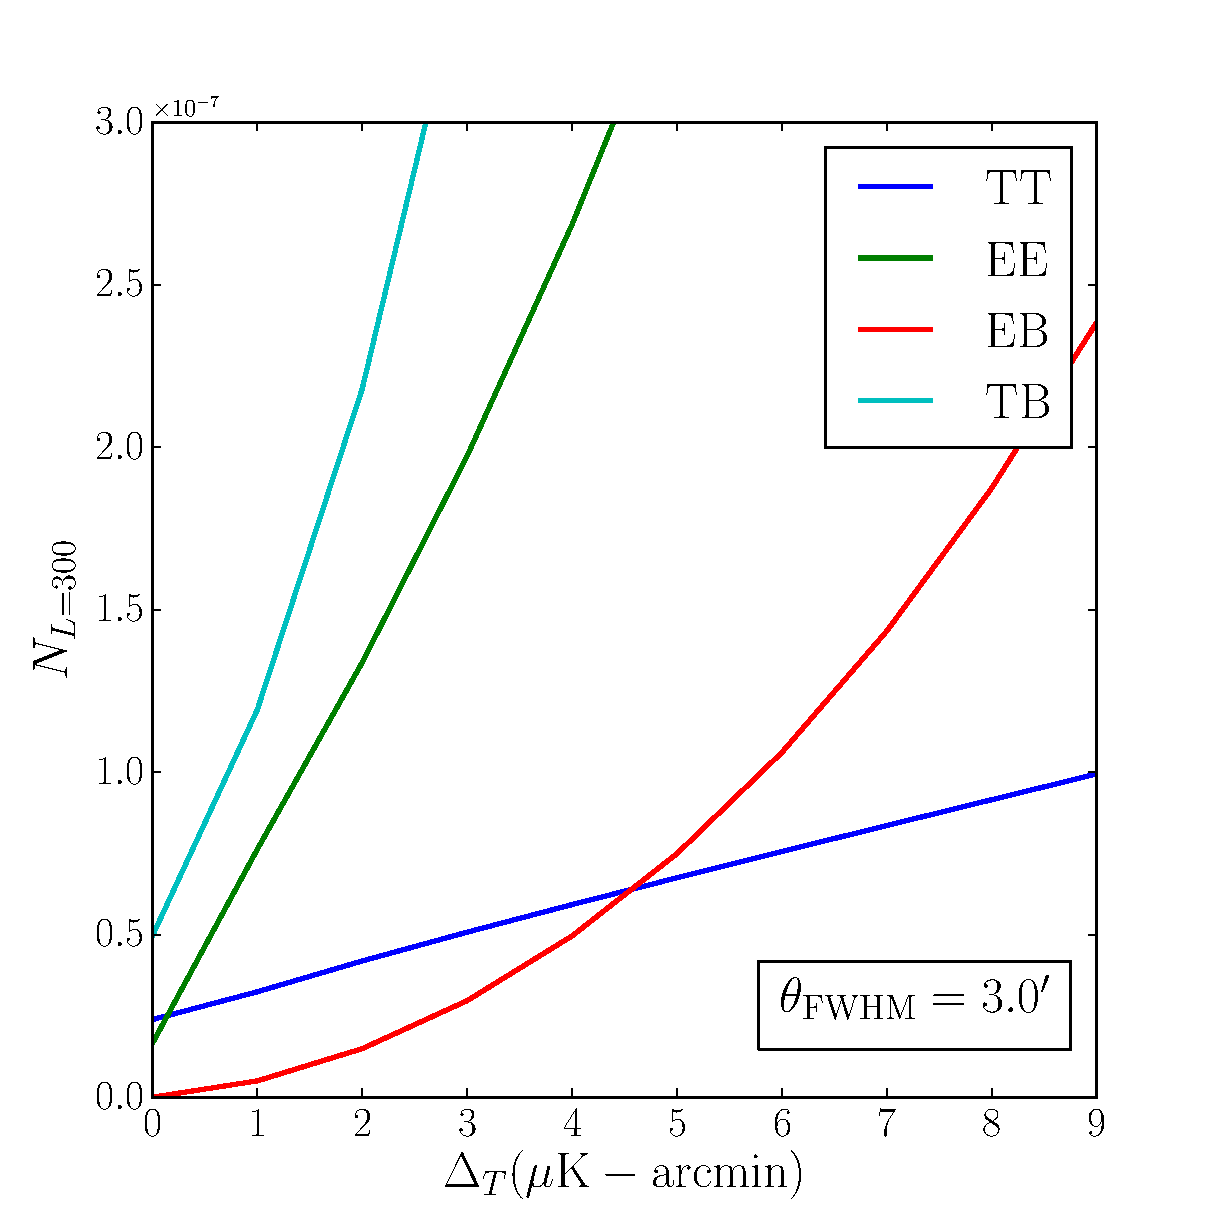
\includegraphics[width=0.45\textwidth]{CMBLensing/ell300_3_00.pdf}
\caption{Noise per mode in the lensing field for different lensing estimators at $L = 300$.  Left panel is for 1.4 arcmin resolution, and right panel is for 4 arcmin resolution.  For a 1.4 and 4 arcmin resolution experiment, the EB polarization estimator yields lower noise than the temperature estimator, below 3uk-arcmin and 5uk-arcmin noise in temperature respectively.}
\label{crossoverPlot}
\end{figure}

However, the primary reason for the increased power of CMB-S4 lensing measurements is this experiment's ability to measure CMB polarization with unprecedented sensitivity. To date, CMB lensing results have had their signal-to-noise dominated by lensing reconstructions based on CMB temperature data (see Figure \ref{n0s_s4}). Such lensing measurements in temperature are limited for two reasons. First, they are limited by systematic biases from astrophysical foregrounds and atmospheric noise. Second, the signal-to-noise on lensing measurements from temperature is intrinsically limited by the cosmic variance of the unlensed CMB temperature field. Due to the unprecedented sensitivity of CMB-S4, the bulk of the lensing signal-to-noise will now be derived from CMB polarization data (see Figures \ref{n0s_s4} and \ref{crossoverPlot}).  Polarization lensing reconstruction will allow CMB-S4 to overcome both of these limitations. For the former, the challenges of astrophysical emission and atmospheric noise are much reduced in polarization data. For the latter, low-noise polarization lensing measurements are not limited by primordial CMB cosmic variance, because they make use of measurements of the B-mode polarization, which contains no primordial signal on small scales. To fully exploit the lack of limiting primordial signal in the B-mode polarization, maximum likelihood lensing reconstruction algorithms can be used, which use iteration to surpass the quadratic estimator. This iterative lensing reconstruction procedure is discussed in more detail in Section \ref{delens}.   


\subsection{Lensing Power Spectrum}\label{kappaPower}

The power spectrum of reconstructed CMB lensing maps is a measure of the matter power spectrum integrated over redshift.  The lensing power spectrum has a broad redshift response kernel, with most of the contribution coming from $z\sim 1-5$, with a peak at $z\sim 2$ (see Figure \ref{cmb-gal-kernels}).  
%(Figure \ref{fig:cmblens_kernel}).  
Most of the scales probed by the lensing power spectrum are on sufficiently
large scales that they are mainly in the linear regime.  As such, the lensing power spectrum is sensitive to physics which affects the growth of structure on large scales and at high redshift, such as the mass of the neutrinos. 


\begin{figure}[htbp]
\centering
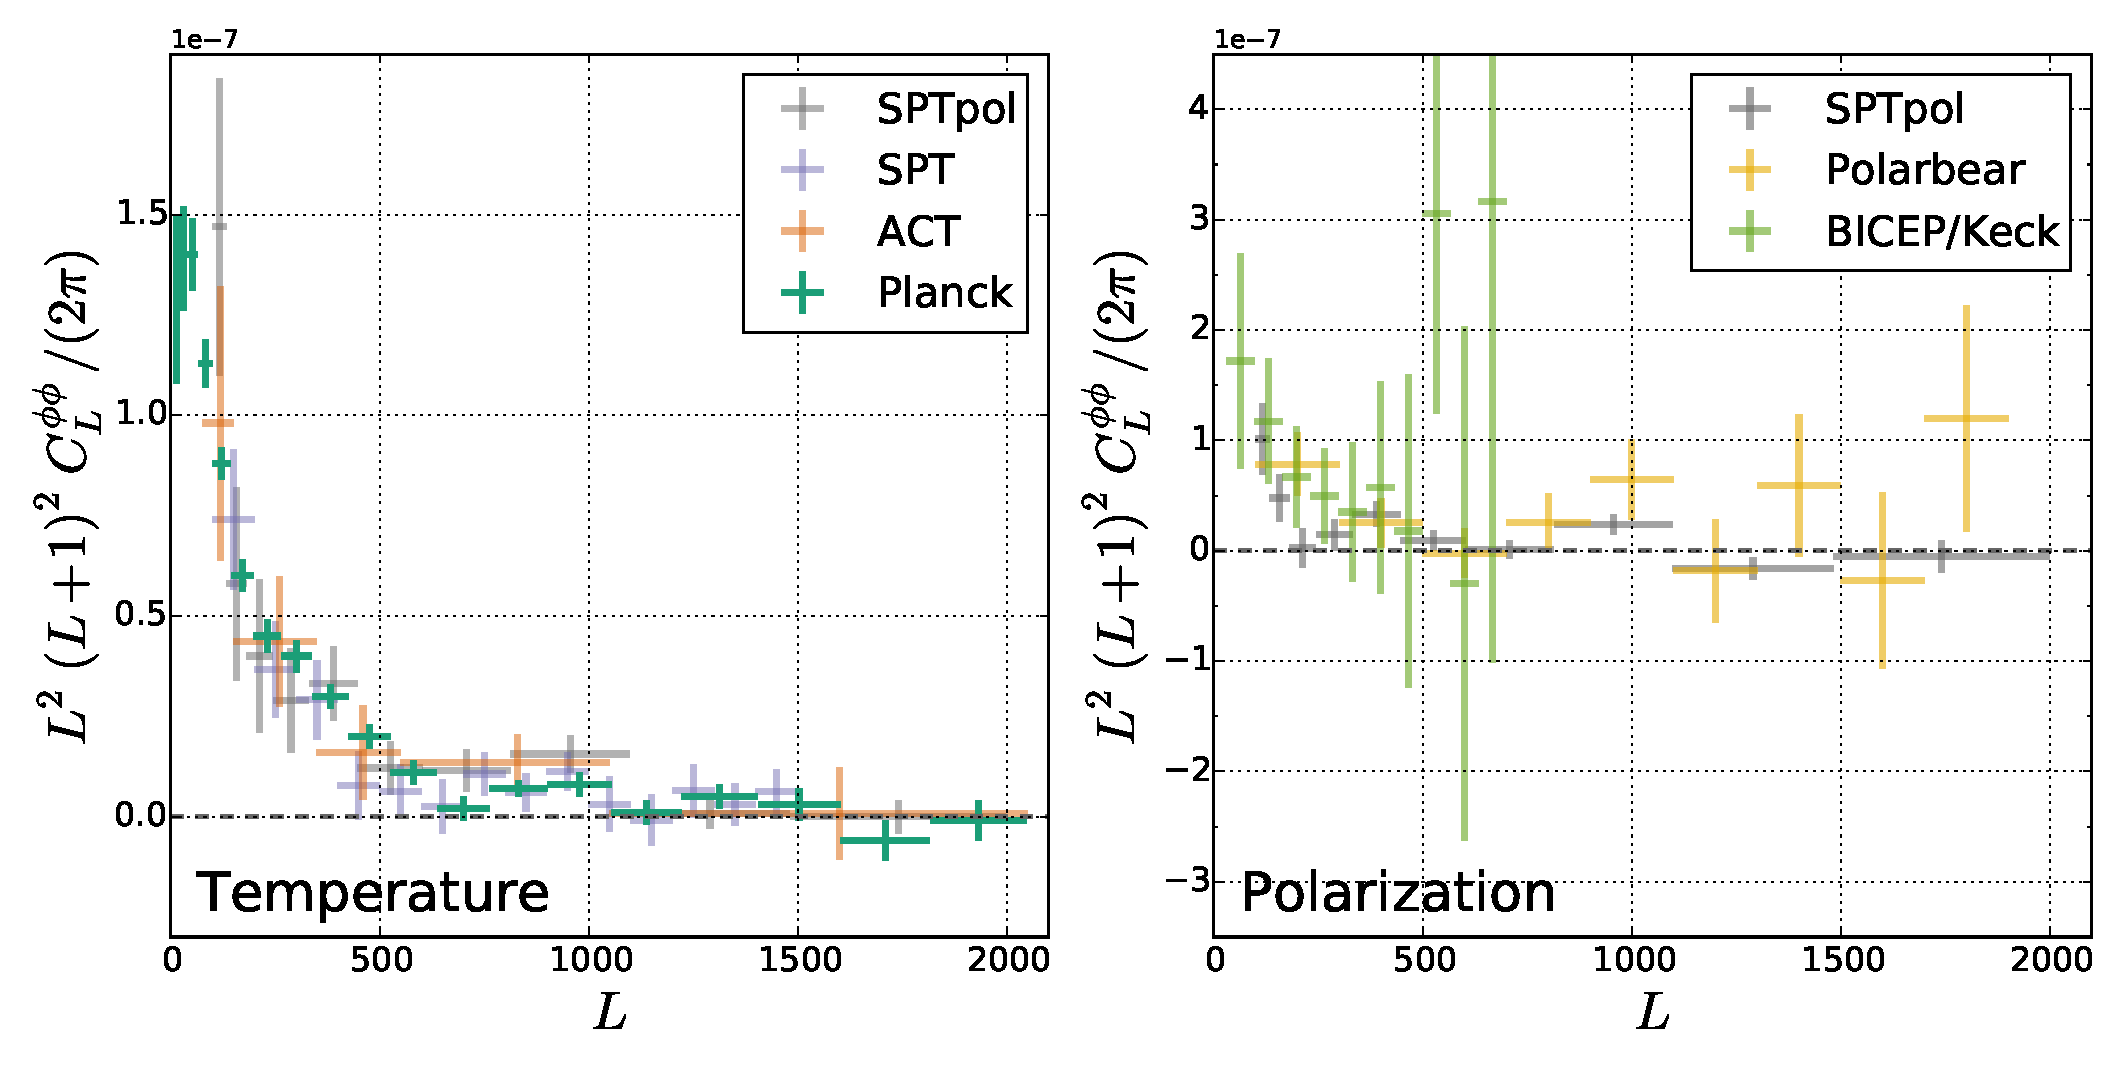
\includegraphics[width=0.9\textwidth]{CMBLensing/autoCompilationTP}
\caption{Compendium of lensing power spectrum measurements since first measurements in 2011.} 
\label{CMBLensPower}
\end{figure}

The latest measurements of the CMB lensing autospectrum, as of early 2016, are shown in Figure \ref{CMBLensPower}. The first detections were obtained by the Atacama Cosmology Telescope (ACT; \cite{Das:2011ak}) and South Pole Telescope  (SPT; \cite{vanEngelen:2012va}) teams, who analyzed maps of several hundreds of square degrees yielding precisions on the lensing power spectrum of approximately 25\% and 18\% respectively.  The Planck collaboration has since provided all-sky lensing maps whose precision on the power spectrum amplitude is approximately 4\% in the 2013 data release and 2.5\% in the 2015 data release.  The first detections of the lensing autospectrum using CMB polarization, which is ultimately a more sensitive measure of lensing for low-noise maps,  have also been obtained (\cite{Ade:2013gez}, \cite{Story:2014hni}, \cite{Array:2016afx}).

There has been rapid improvement in these measurements over the period of just a few years. 
Early detections of the CMB lensing autospectrum were not sample variance limited over a broad range in $L$ and were only covering a relatively small sky area;  
the  power spectrum of the noise in the CMB lensing reconstruction in the 2015 Planck data release is approximately equal to the lensing power spectrum only at its peak of $L \sim 40$, but smaller scales are noise-dominated. Lensing reconstructions from current ground-based surveys (like SPTPol, ACTPol, PolarBear) 
are strongly signal-dominated below $L \sim 200$ and noise-dominated on smaller scales.  However, they have been obtained over relatively small sky areas of several hundreds of degrees. A ground-based survey such as CMB-S4, with wide sky coverage, low-noise, and high resolution, will provide a sample-variance-limited measurement to scales below $L \sim 1000$ (see Figure \ref{n0s_s4}) over a wide area.   
 

\begin{figure}[htbp]
\centering
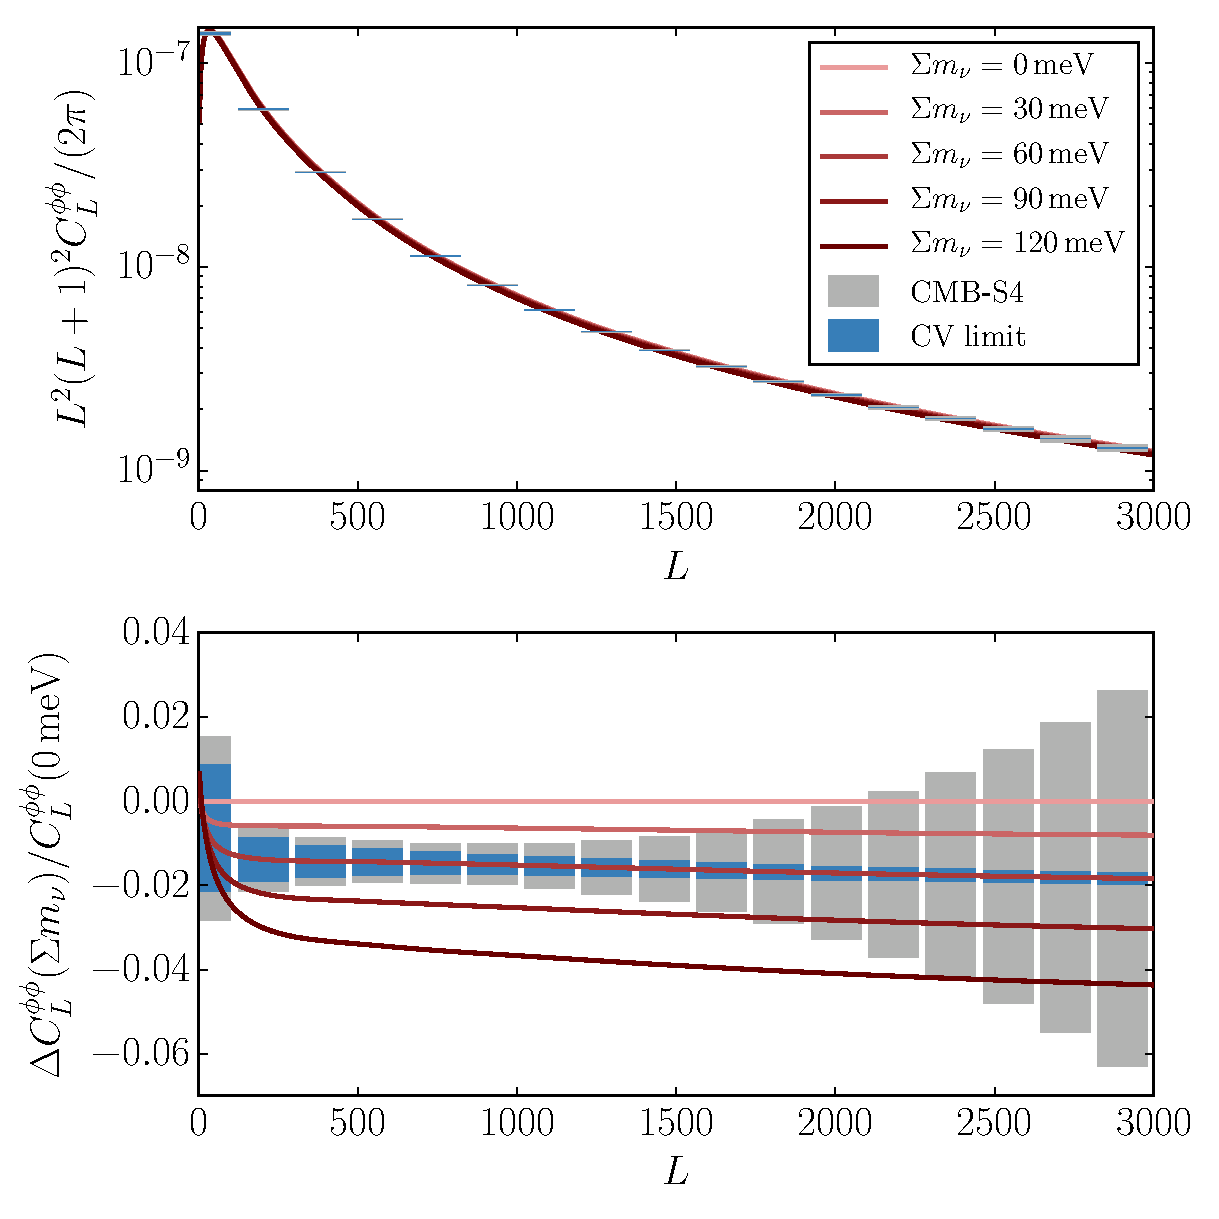
\includegraphics[width=0.85\textwidth]{CMBLensing/mnuS4errors.pdf}
\caption{Constraining neutrino mass with CMB-S4.  Top: lensing power spectra for multiple neutrino masses (curves) together with forecasted errors for S4.  Bottom: residual from curve at zero neutrino mass.  Error boxes are shown centered at the minimal value of $60$\,meV.  S4 will be targeted to resolve differences in neutrino mass of 20\,meV. }
\label{mnuS4errors}
\end{figure}

Such a measurement holds the promise to qualitatively improve our understanding of cosmology.  While the cosmological parameters describing the standard Lambda-Cold Dark Matter model have been precisely measured, extensions to this model can be constrained by including growth or geometrical information at a new redshift.  From the redshifts probed by CMB lensing, extensions to the standard model such as a non-minimal mass for the sum of the neutrinos, a dark energy equation of state deviating from the vacuum expectation, and a non-zero curvature of the Universe can all be probed to much higher precision than with the primordial CMB alone. Figure \ref{mnuS4errors} shows the expected precision of a CMB-S4 lensing power spectrum measurement and demonstrates its potential, for example, to discriminate between different neutrino mass scenarios. 



\section{Cross Correlations with CMB Lensing}\label{cross}

Cross-correlating CMB lensing maps with other probes of large-scale structure provides a powerful source of information inaccessible to either measurement alone. Because the CMB last-scattering surface is extremely distant, the CMB lensing potential includes contributions from a wide range of 
intervening distances extending to high redshift. As a result, many other cosmic observables trace some of the same large-scale structure that lenses the CMB. These cross-correlations can yield high-significance detections, are generally less prone to systematic effects, and given the generally lower redshift distribution of the other tracers, are probing large-scale structure in exactly the redshift range relevant for dark energy studies (see Figure \ref{cmb-gal-kernels}). 
With CMB-S4, cross-correlations will transition from detections to powerful cosmological probes. 

\begin{figure}[htbp]
\centering
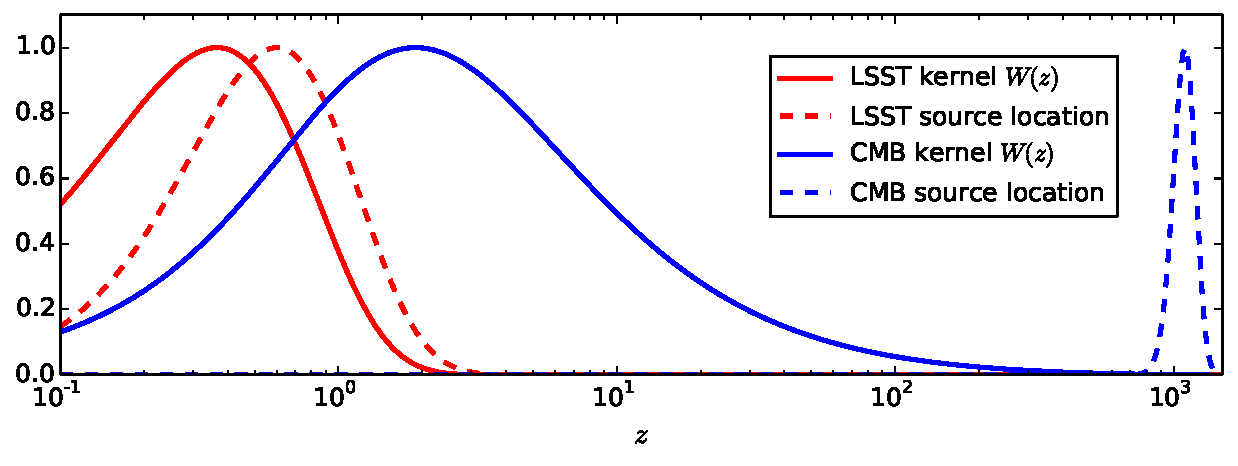
\includegraphics[width=0.85\textwidth]{CMBLensing/CMB_effs.pdf}
\caption{Redshift kernel for CMB lensing (blue solid) and for cosmic shear with LSST (red solid), together with the expected redshift distribution of LSST galaxies (red dashed) and the CMB source redshift (blue dashed).}
\label{cmb-gal-kernels}
\end{figure}

\subsection{CMB Lensing Cross Galaxy Density}
Galaxies form in the peaks of the cosmic density field; thus the distribution of galaxies traces the underlying dark matter structure.  This same dark matter structure also contributes to the CMB lensing potential.
Cross-correlating galaxy density distributions with CMB lensing is thus a powerful probe of structure and is highly complementary to galaxy clustering measurements.
Galaxy surveys measure luminous matter while CMB lensing maps directly probe the underlying dark matter structure. Thus these cross-correlations provide a clean measurement of the relation between luminous matter and dark matter.
Cross-correlations between independent surveys are also more robust against details of selection functions or spatially inhomogeneous noise that could add spurious power to auto-correlations.
Additionally, while CMB lensing maps are projected along the line-of-sight, galaxy redshift surveys provide information about the line-of-sight distance; thus cross-correlating redshift slices of galaxy populations allows for tomographic analysis of the CMB lensing signal (see, e.g., \cite{Baxter:2016ziy}, \cite{Miyatake:2016gdc}).
These benefits can lead to improved constraints on cosmology: for example, with LSST galaxies, it has been shown that including cross-correlation with CMB lensing can substantially improve constraints on neutrino masses (\cite{Pearson:2013iha}).


CMB lensing was first detected using such a cross-correlation (\cite{Smith:2007rg}, \cite{Hirata:2008cb}).  Since these first detections, cross-correlation analyses have been performed with tracers at many wavelengths, including optically-selected sources (\cite{Bleem:2012gm}, \cite{Sherwin:2012mr}, \cite{Ade:2013tyw}, \cite{Baxter:2016ziy}, \cite{Pullen:2015vtb}), infrared-selected sources (\cite{Bleem:2012gm}, \cite{Geach:2013zwa}, \cite{DiPompeo:2014yea}), sub-mm-selected galaxies (\cite{Bianchini:2014dla}) and maps of flux from unresolved dusty star-forming galaxies (\cite{Holder:2013hqu}, \cite{Hanson:2013daa}, \cite{Ade:2013aro}, \cite{vanEngelen:2014zlh}). 

These cross-correlations between CMB lensing and galaxy clustering have already been used to test key predictions of general relativity, such as the growth of structure (\cite{Baxter:2016ziy}) as a function of cosmic time, and the relation between curvature fluctuations and velocity perturbations (\cite{Pullen:2015vtb}). Cross-correlations using CMB-S4 lensing data will enable percent level tests of general relativity on cosmological scales.

On the timescale of the CMB-S4 experiment, a number of large surveys are expected be concurrent or completed, including DESI, WFIIRST, Euclid, and LSST.  Due to the high number density of objects detected, wide area coverage, and accurate redshifts, the precision of cross-correlation measurements with these surveys will be much higher than those performed to date.  For example, the amplitude of cross-correlation between the CMB-S4 convergence map and the galaxy distribution from LSST is expected to be measured to sub-percent levels.  


\subsection{CMB Lensing Cross Galaxy Shear}\label{lensxlens}


There have been several recent detections of the cross-correlation between lensing of the CMB and galaxy shear (\cite{Hand:2013xua}, \cite{Liu:2015xfa}, \cite{Kirk:2015dpw}), demonstrating the emergence of a new cosmological tool. In addition, CMB and galaxy lensing can be combined with galaxy surveys for lensing tomography measurements, providing the ability to reconstruct the 3D mass distribution. CMB lensing offers similar signal-to-noise as galaxy shear surveys but provides the most distant source possible, allowing this 3D reconstruction to extend to the edge of the observable universe and providing a high-redshift anchor for dark energy studies.  The combination of CMB and galaxy lensing with galaxy surveys can also be used to measure cosmographic distance ratios (\cite{Miyatake:2016gdc},\cite{Singh:2016xey}), which provides a clean, complementary probe of the geometry of our Universe and dark energy. 

CMB lensing can also be used as an external calibration for galaxy shear studies. It has been shown (\cite{Vallinotto:2011ge}, \cite{Vallinotto:2013eva}, \cite{Das:2013aia}) that CMB lensing, galaxy clustering, and galaxy shear data taken together can in principle cross-calibrate each other while still providing precise constraints on cosmological parameters. This has been successfully applied to existing surveys (\cite{Liu:2015xfa}, \cite{Baxter:2016ziy}, \cite{Miyatake:2016gdc}, \cite{Singh:2016xey}) as a proof of principle. CMB-S4 can be expected to provide an important systematics check on galaxy shear surveys such as WFIRST, Euclid, and LSST. 

\subsection{CMB Halo Lensing}\label{haloLensing}

In addition to constructing CMB lensing maps of matter fluctuations on relatively large scales ($> \sim 5$ arcmin) as discussed in the preceding sections, one can also make CMB lensing maps capturing arcminute-scale matter distributions. Such small-scale measurements capture lensing of the CMB by individual dark matter halos, as opposed to lensing by larger scale structure represented by the clustering of halos.  This small-scale lensing signature, called CMB halo lensing, allows one to obtain measurements of the mass of these halos.  

\begin{figure}[htbp]
\centering 
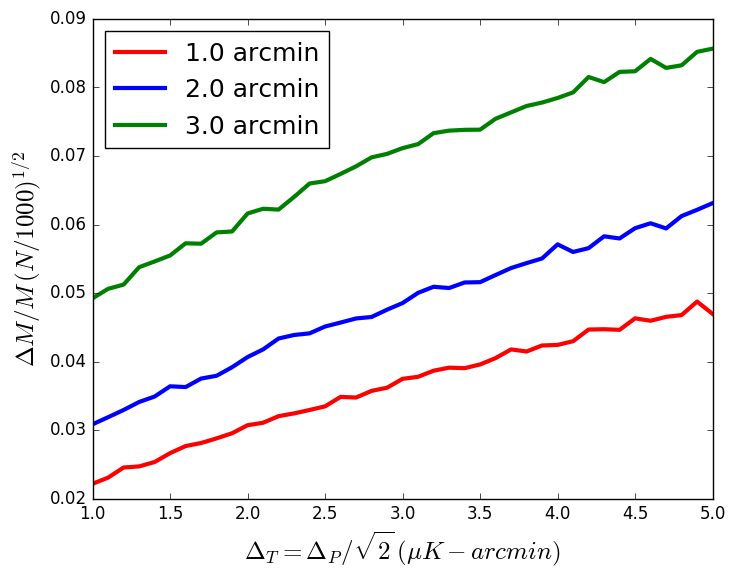
\includegraphics[width=0.65\textwidth]{CMBLensing/HaloLens.png}
\caption{Mass uncertainty from CMB halo lensing measurements stacking $10^3$ halos of mass $M_{180\rho_{m_0}} \approx 5\times 10^{14} M_{\odot}$, as a function of instrumental noise and varying instrumental resolution.}
\label{haloLens}
\end{figure}

Using CMB halo lensing, CMB-S4 will be sensitive to halo masses in the range of $10^{13} M_{\odot}$ to $10^{15} M_{\odot}$.  This corresponds to halos belonging to galaxy groups and galaxy clusters.  Measuring the abundance of galaxy clusters as a function of mass and redshift provides a direct handle on the growth of matter perturbations and consequently, on the equation of state of dark energy.  Galaxy clusters can be identified internally in CMB maps through their wavelength-dependent imprint caused by the thermal Sunyaev-Zeldovich (tSZ) effect.  This technique provides a powerful redshift-independent way of detecting clusters. However, the scaling between the tSZ observable, which is sensitive to baryonic physics, and the cluster mass, which is dominated by dark matter is not precisely constrained.  Calibration of this mass scaling and scatter is currently the dominant systematic for extracting dark energy constraints from cluster abundance measurements. 

Weak lensing of galaxies behind the galaxy cluster is a promising method for mass calibration since it is directly sensitive to the total matter content of the cluster.  Reconstructing the mass profiles of clusters using measurements of the shapes of distant galaxies in deep photometric surveys is an active research program; however, it is often limited by the poor accuracy of source redshifts and the availability of sufficient galaxies behind the cluster, especially for very high-redshift clusters. CMB halo lensing has an advantage here since the CMB is a source of light which is behind every cluster, has a well defined source redshift, and well understood statistical properties.  

A general approach for obtaining the average mass of a sample of clusters using CMB halo lensing is to reconstruct the lensing deflection field using a variation of the standard quadratic estimator, stack the reconstructed lens maps at the positions of the clusters, and fit the resulting signal to a cluster profile (e.g NFW). A modified quadratic estimator is used to reconstruct small-scale lensing signals since the standard estimator tends to underestimate the signal from massive clusters (\cite{Hu:2007bt}).  This modified estimator makes use of the fact that halo lensing induces a dipole pattern in the CMB that is aligned with the background gradient of the primordial CMB.  The halo lensing signal can be measured with both temperature and polarization estimators, which can be used to cross check each other and reduce systematics. 

CMB experiments have only very recently reached the sensitivity required to detect the lensing signal on scales of dark matter halos.  The first detections were reported in 2015 by ACTPol (\cite{Madhavacheril:2014slf}), SPT (\cite{Baxter:2014frs}), and Planck (\cite{Ade:2015fva}).  CMB-S4 will be capable of providing precision mass calibration for thousands of clusters which will be an independent cross check of galaxy shear mass estimates and will be indispensable for high-redshift clusters. Figure \ref{haloLens} shows that an arcminute resolution experiment with a sensitivity of around 1$\mu$K-arcmin can determine the mass of 1000 stacked clusters to $\sim 1\%$ precision, combining temperature and polarization maps. The primary systematic in temperature maps is contamination from the thermal SZ effect and radio and infrared galaxies coincident with the halos. This systematic can be mitigated using multi-frequency information due to the spectral dependence of the thermal SZ effect and galaxy emission, a procedure that requires the high sensitivity at multiple frequencies allowed by CMB-S4.  Halo lensing from polarization maps is relatively free of these systematics, and ultimately may be the cleanest way to measure halo masses.  This requires the high polarization sensitivity provided by CMB-S4. 


\section{Delensing}\label{delens}

To probe an inflationary gravity wave signal it is important to have low-noise B-mode polarization maps. However, for instrumental noise levels below $\Delta_P \simeq 5 \mu$K-arcmin in polarization, the dominant source of noise is no longer instrumental, but instead is from the generation of B-mode polarizationby lensing of E-mode polarization from recombination (see Figure \ref{snowmssDelens}).  This B-mode lensing signal has a well-understood amplitude, but the sample variance in these modes in the CMB maps leads to increased noise in estimates of the inflationary B-modes. Unlike other sources of astrophysical B-mode fluctuations in the map, it cannot be removed with multifrequency data.  Fortunately, this signal can be removed using map-level estimates of both the primordial $E$-mode map and the CMB lensing potential $\phi$ with a technique called delensing. However, this procedure requires
precise maps of both the E-modes and of the gravitational lensing potential
(which can be obtained from the CMB-S4 data itself).

\begin{figure}[htbp]
\centering
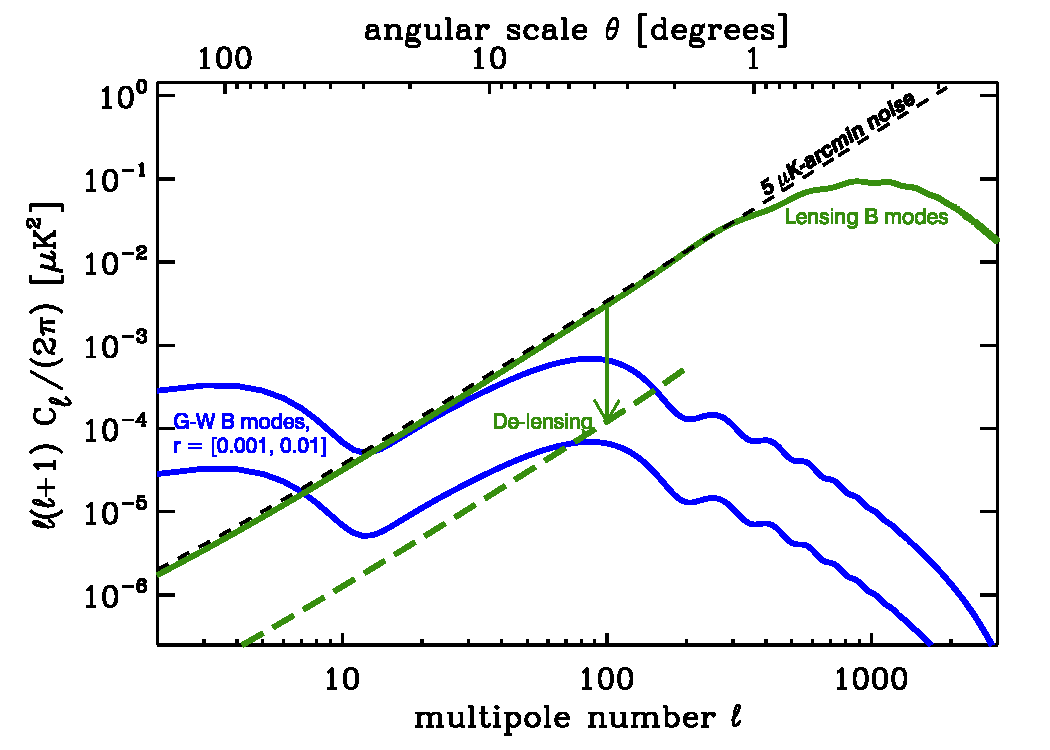
\includegraphics[width=0.65\textwidth]{CMBLensing/cmb_powspec_for_s4scibooklensing.pdf}
\caption{The green curve is the power spectrum of lens-induced $E$-to-$B$ mixing.  Delensing can reduce the amplitude of this effect by large factors (green dashed curve) yielding lower effective noise in $B$-mode maps.}
\label{snowmssDelens}
\end{figure}

Moreover, delensing will be a crucial part of the reconstruction of the CMB lensing field for CMB-S4, even for science goals like measuring the neutrino mass.  This is because at low noise levels the standard quadratic reconstruction of lensing using the $EB$ estimator (\cite{Hu:2001kj}) can be improved upon by cleaning the B-mode CMB maps of the lens-induced $B$-mode fluctuations and then performing lens reconstruction again.  This procedure can be repeated until CMB maps cleaned of the lensing signals are produced (see Figure \ref{iterative}).  

\begin{figure}[htbp]
\centering
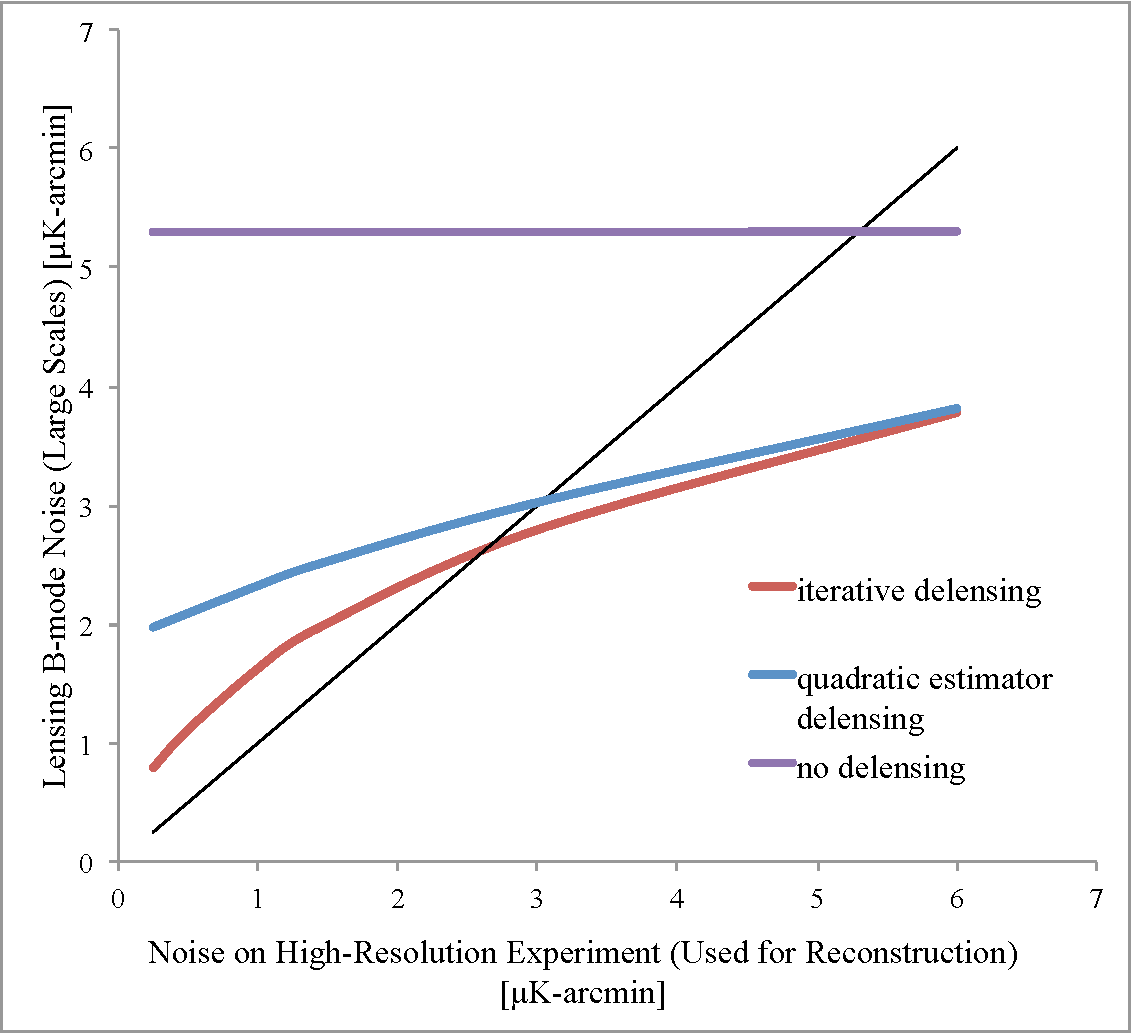
\includegraphics[width=0.60\textwidth]{CMBLensing/delensPlot.pdf}
\vspace{0.3cm}
\caption{The $B$-mode noise on large scales as a function of the noise level used in $EB$-based lens reconstruction.  The purple line is for no delensing and shows that lens-induced  $E$ to $B$ mixing manifests as an effective 5 uK-arcmin white noise level.  The blue curve shows the improvement possible when using a lens reconstruction to remove this source of effective noise.  The red curve shows further improvement when the delensing is performed in an iterative fashion.}
\label{iterative}
\end{figure}

Delensing in principle can be a nearly-perfect procedure: in the limit of no instrumental noise or primordial $B$ modes, the lensing potential and the primordial $E$-mode map can be nearly-perfectly imaged (\cite{Hirata:2003ka}).  However, the finite noise in a CMB-S4 survey will lead to residual lensing $B$ modes which cannot be removed and will act as a noise floor for studying primordial B-modes from tensors.  In addition, higher order effects may ultimately limit the reconstruction.


It is important to have relatively high-angular resolution maps in order to obtain the small-scale $E$ and $B$ fluctuations needed for the $EB$ quadratic lensing estimator.  As shown in Figure \ref{sigCon}, quadratic EB lens reconstruction requires high-fidelity measurements of the E and B polarization fields on a variety of angular scales.  For large-scale lenses, such as those at degree scales of $L=300$, the E and B fields contain information to scales of several arcminutes ($l \sim 2000$).  For arcminute-scale lenses at $L = 2000$, the B field must be measured to even smaller scales, $l > 3000$. 

\begin{figure}[htbp]
\centering
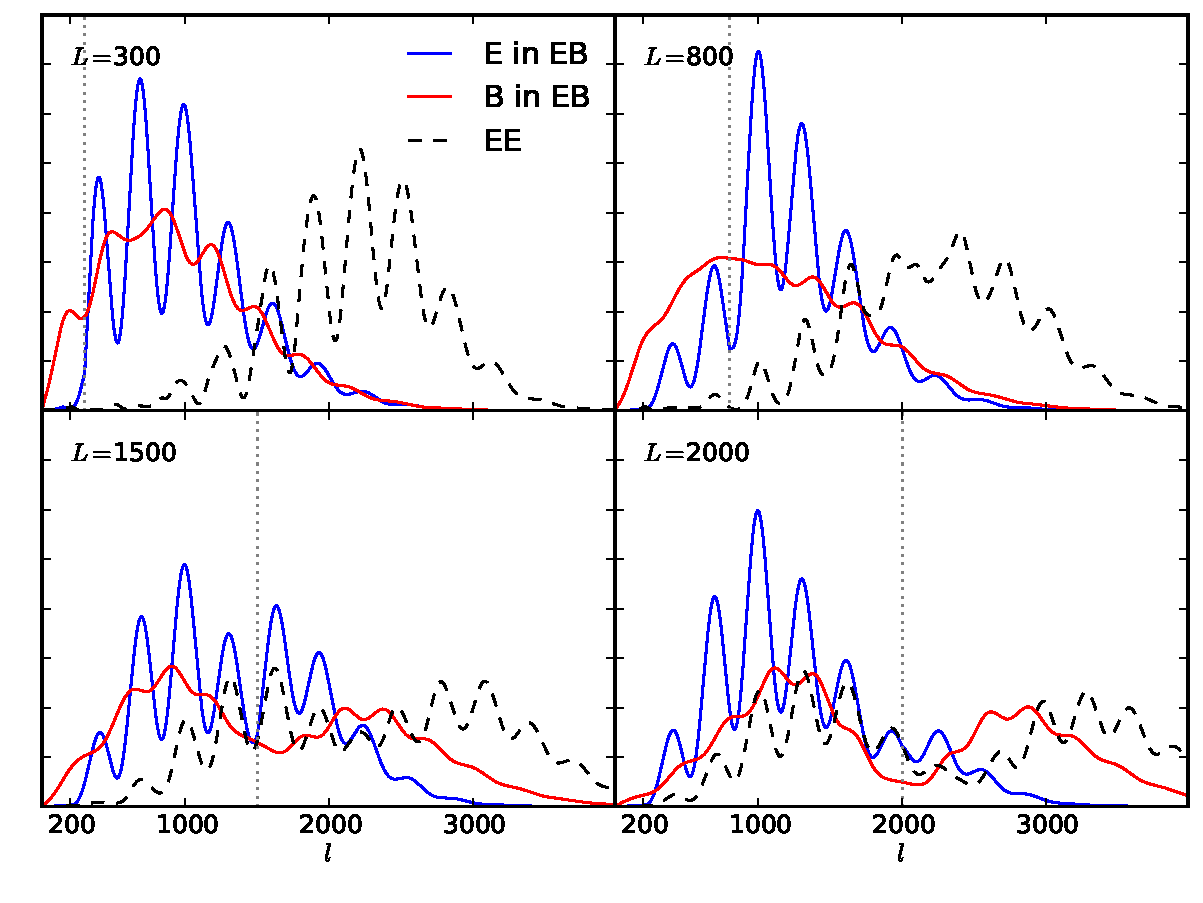
\includegraphics[width=0.65\textwidth]{CMBLensing/signal_contribs.pdf}
\caption{Contributions from CMB scales ($\ell$) to lensing reconstruction on four lensing scales ($L$).  The $EB$ estimator is expected to be the main channel for lensing science with CMB-S4.  On degree and sub-degree scales, $L = 300$ and $800$, the estimator uses E and B modes at $\ell \sim 1000$.  On scales of several arcmin, $L = 1500$ and $2000$, the estimator uses B modes on significantly smaller scales.  Figure taken from Pearson et al. 2014}
\label{sigCon}
\end{figure}

Potential systematic biases with the delensing procedure are similar to those for measuring the lensing power spectrum. The impact of polarized dust and polarized synchrotron emission from the Galaxy as well as the impact of polarized extragalactic emission on the reconstructed lensing field are discussed in Section \ref{systAst} as well as ways to mitigate them.

Additionally, rather than using an estimate of the CMB lensing field obtained internally from the CMB itself, it is also possible to use other tracers of large-scale structure which are correlated with  CMB lensing (\cite{Smith:2010gu}).  In particular the dusty, star-forming galaxies that comprise the cosmic infrared background (CIB) are strongly correlated with CMB lensing due to their redshift distribution which peaks near $z \sim 2$ (\cite{Sherwin:2015baa}, \cite{Simard:2014aqa}).  The level of correlation can be as high as $80\%$ (\cite{Ade:2013aro}) and can in principle be improved using multifrequency maps of the CIB which select different emission redshifts (\cite{Sherwin:2015baa}). However, as shown in (\cite{Smith:2010gu}), the gain from delensing with external galaxy tracers is modest, and delensing internally with CMB maps holds far more promise.


\section{Systematic Effects and Mitigation}\label{syst}
The quadratic estimators used for lens reconstruction search for departures from statistical isotropy.  The lens effect locally changes the CMB power spectrum via shear and dilation effects (e.g. \cite{Bucher:2010iv}).  Other sources of deviation from statistical isotropy can thus be confused with lensing effects; these can be of both instrumental and astrophysical origin.

\subsection{Astrophysical Systematics}\label{systAst}
	
Extragalactic sources and tSZ clusters in temperature maps can be troublesome for lensing estimates in two ways: they tend to cluster more strongly in overdense regions (i.e, are non-Gaussian), an effect which
lensing estimators can mistakenly attribute to lensing, while individual sources show up as strong local deviations from statistical isotropy.  

Planck (\cite{Ade:2013tyw}) had to remove the effect of Poisson sources biasing the CMB lensing power spectrum, which left untreated would have shifted their measured lensing power spectrum amplitude by $4\%$, a  1$\sigma$ shift.  For an experiment with lower map noise level and smaller beam, such as CMB-S4, sources can be found and removed to much fainter flux thresholds, making this a much smaller effect.  The largest sources of bias thus come from the three-point and four-point correlation functions of the non-Gaussian clustering of sources and non-Gaussian clustering between the sources and the lensing field.  These biases can be as large as several percent (\cite{vanEngelen:2013rla}, \cite{Osborne:2013nna}) and their amplitude is highly model-dependent in temperature-based CMB lensing estimates. However, the extragalactic sources and tSZ clusters that can cause large sources of bias in temperature-based CMB lensing estimates are expected to be nearly unpolarized and therefore not a concern for polarization-based lensing estimates. In
addition, sensitive multi-frequency temperature measurements should be able to spectrally remove these foregrounds through their unique frequency
signatures. In addition, a robust campaign to measure these non-Gaussianities in the CMB data should allow a careful empirical understanding of these
effects, an approach known as ``bias-hardening'' (\cite{Osborne:2013nna}).  

Observed levels of the polarization fraction of the diffuse Galactic emission at intermediate and high latitudes, reaching $10\%$ or more, 
have been shown to impact non-negligibly on quadratic estimators for lensing extraction (\cite{Fantaye:2012ha}). 
This is due to leakage of the dominating long wavelength modes of the foreground signal onto the scales at which the lensing pattern is reconstructed. 
Therefore, as was the case for the Planck data analysis (\cite{Ade:2015zua}), lensing extraction has to be validated on foreground cleaned maps output from a component separation process. 

\subsection{Instrumental and Modeling Systematics}\label{systInst}
 	
Given the unprecedented precision targeted by CMB-S4 lensing measurements, the effects of instrumental systematic errors must be investigated and well-controlled. Since lensing results in a remapping or distortion of the sky, beam systematics are a particular concern. 

The main beam systematics that affect CMB measurements are commonly described by differential gain, differential beamwidth, differential ellipticity, as well as differential pointing and rotation. In Smith et al.~2003, the impact of all these beam systematics on lensing measurements and hence on $r$ and $\sum m_\nu$ was investigated using a Fisher matrix formalism. It was found that for a CMB-S4-type experiment, with $1 \mu $K-arcmin noise and a 3 arcmin beam, the beam characterization from planets or other point sources will be sufficiently accurate that the biases arising from differential gain, differential beamwidth and differential ellipticity are less than one tenth of the one-sigma error on key parameters. Differential pointing and rotation must be controlled to within 0.02 arcmin and 0.02 degrees respectively in order to be similarly negligible.

While ideally the instrument can be designed or shown using measurements to have systematic errors that are negligible, one can also estimate residual beam systematics directly from the data, in a manner analogous to bias-hardening. Many beam systematics result in a known mode-coupling (\cite{Yadav:2009eb}).  Their levels can hence be estimated by quadratic estimators and projected out, though complications due to the scan strategy must be accounted for. This method of beam-hardening was first demonstrated in Planck (2013).

Another challenge in making high precision lensing power spectrum measurements is predicting the actual observed lensing power spectrum, given a set of cosmological parameters. One example of such a challenge is the presence of higher-order biases, which have been previously neglected in theory calculations. For instance, often the Gaussianity of the lensing potential is assumed; however, if the full large scale structure non-linearity is taken into account, biases result that can affect measurements at the one-sigma level over many bandpowers. In this respect, the modeling of ray tracing through N-body simulations (\cite{Calabrese:2014gla}) represents a resource for accounting for the complexity of this non-linearity.


In addition, the lensing power spectrum itself may not be exactly known, due to baryonic effects which modify the mass distribution. While this is a challenge for optical weak lensing measurements, investigations with simulations have found that such baryonic effects can be neglected for CMB lensing, at least at the precision achievable by CMB-S4 (\cite{Natarajan:2014xba}).

\section{Impact of CMB Lensing/Delensing on Parameters}\label{forecasts}

Measurements of CMB lensing are essential to all the key science goals of CMB-S4.  Since CMB lensing is a sensitive probe of the matter power spectrum, CMB lensing measurements added to measurements of the primordial CMB power spectrum serve to significantly tighten parameter constraints.  In particular, measurements of the CMB lensing power spectrum (4-point signal) and the peak-smearing lensing induces in the CMB primordial power spectrum (2-point signal) yield tight constraints on the sum of the masses of the neutrinos ($\sum {m_\nu}$).  
\begin{figure}[htbp]
\centering
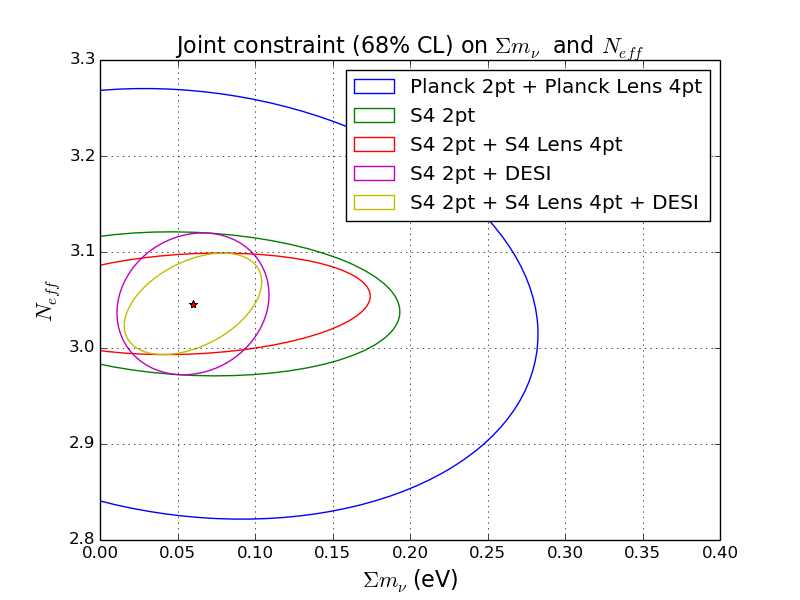
\includegraphics[width=0.7\textwidth]{CMBLensing/Neff_Mnu.png}
\caption{CMB lensing signals measured both from lensing-induced mode coupling in the CMB power spectrum (2-point function) and from the CMB lensing power spectrum (4-point function) drive the constraint on the sum of the neutrino masses.  The constraint on the number of relativistic species is improved by about 30\% after delensing the E-mode power spectrum using 4-point lensing information.}
\label{neutrinos}
\end{figure}
Cross-correlations of CMB lensing maps with maps of galaxy density and galaxy shear can provide tight constraints on curvature, the dark energy equation of state ($w$), and modified gravity.  Delensing B-mode and E-mode polarization maps can also give strong constraints on the tensor-to-scalar ratio ($r$) from inflationary primordial gravity waves, as well as tighten constraints on the number of neutrino species ($N_{\rm{eff}}$).  

\begin{figure}[htbp]
\centering
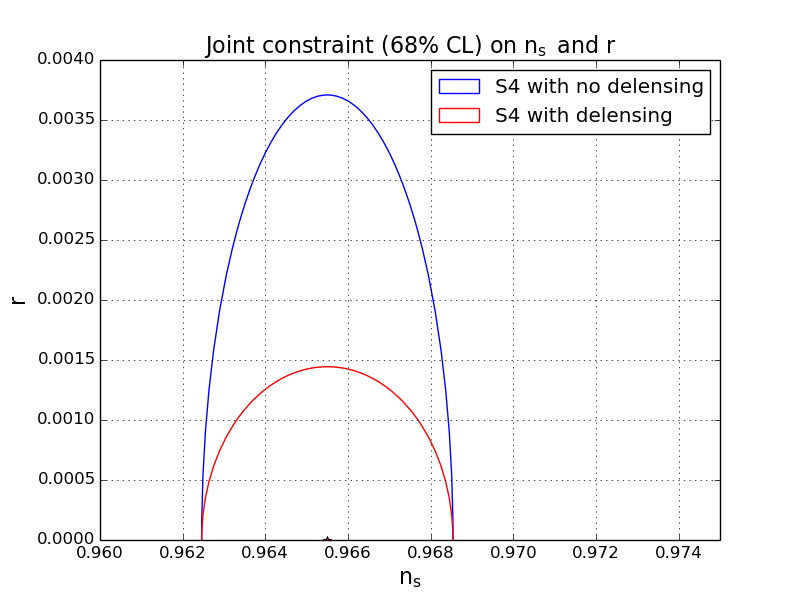
\includegraphics[width=0.45\textwidth]{CMBLensing/inflation.png}
\caption{Delensing is critical to achieving the tightest constraints on $r$.  The impact of delensing on $r$ is also more significant as the sensitivity of the experiment is increased. For representive CMB-S4 map sensitivites, iterative delensing can improve the constraint on $r$ by roughly a factor of 2.5.}
\label{inflation}
\end{figure}


Figures \ref{neutrinos}-\ref{darkEnergy} show the importance of CMB lensing for measuring key cosmological parameters.  Figure \ref{neutrinos} shows constraints on $\sum {m_\nu}$ and $N_{\rm{eff}}$ including the lensing signals from the 2-point and 4-point functions.  In particular for $\sum {m_\nu}$, there is almost no constraining power on $\sum {m_\nu}$ from the primordial CMB power spectrum, so the constraint on $\sum {m_\nu}$ is driven by the lensing-induced mode coupling in the 2-point function and from the 4-point lensing signal.  

For Figure \ref{neutrinos}, no foregrounds are assumed and only white instrumental noise.  Since most of the lensing signal-to-noise is coming from the EB lensing estimator (see Figure \ref{crossoverPlot}), white noise may be a reasonable assumption if leakage of atmospheric noise in temperature maps into polarization maps can be prevented via a half-wave plate or some alternative.  This Figure also assumes that CMB-S4 will observe $40\%$ of the sky, and Planck primordial CMB data is included in the non-overlapping region of the sky ($65\% - 40\% = 25\%$ of sky).  For both CMB-S4 and Planck, temperature modes between $l=50-3000$ and polarization modes between $l=50-5000$ are used.  Planck low-ell data between modes $l=2-50$, and lensing modes between $L=40-3000$ are also included.  Here the 2-point CMB power spectrum is iterativley delensed to get tighter parameter constraints, and the covariance between the residual lensing in the 2-point function and the lensing in the 4-point signal is taken into account.     

\begin{figure}[htbp]
\centering
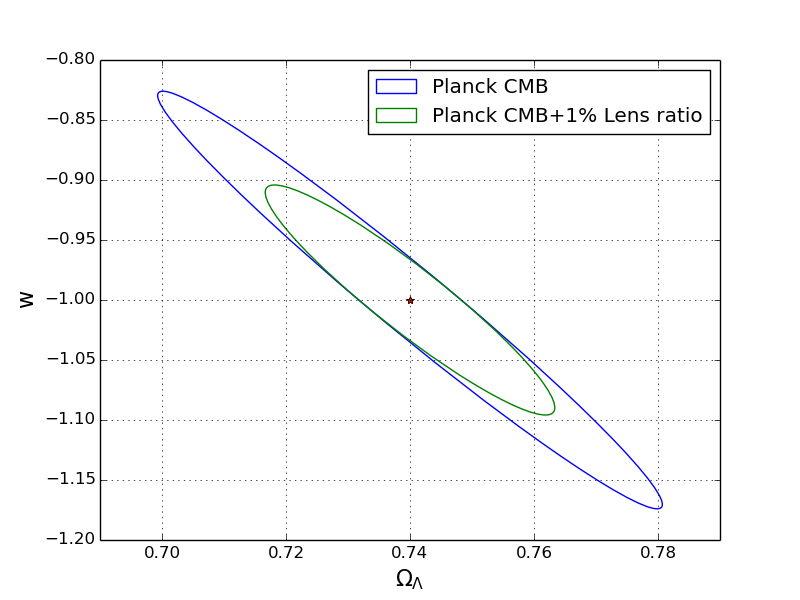
\includegraphics[width=0.65\textwidth]{CMBLensing/Das_confEllipse_omL_w_1sigma.png}
\caption{The improvement in dark energy parameters adding a 1\% measurement of the cosmographic distance ratio (see Section \ref{lensxlens}), obtained from the combination of CMB-S4 lensing, LSST shear, and DESI galaxy survey data, to Planck CMB data.}
\label{darkEnergy}
\end{figure}

In Figure \ref{inflation} the impact of delensing on measuring the tensor-to-scalar ratio $r$ is shown.  This Figure assumes the same instrument configuration and foreground-cleaned map depths as discussed in chapters 2 and 8 for a survey covering 10\% of the sky.  Delensing the B-mode power spectrum using a lensing reconstruction made from E-mode and B-mode maps, increases the senstivity to $r$ by a factor of 2.5.  For deeper effective maps depths, the improvement on the $r$ constraint from delensing is even larger (see Figure \ref{iterative}).  For a $1 \mu $K-arcmin effective map depth, for example, iterative delensing improves the constraint on $r$ by a factor of five.  

Figure \ref{darkEnergy} shows the constraints on dark energy from CMB-S4 obtained largely from the cross-correlation of CMB lensing with other lower-redshift probes of large-scale structure.  Here is shown the improvement when a 1\% measurement of the cosmographic distance ratio (see Section \ref{lensxlens}), obtained from the combination of CMB-S4 lensing, LSST shear, and DESI galaxy survey data, is combined with Planck CMB data.  This is just one example of a number of cross-correlations with CMB-S4 lensing that can constrain the geometry of the Universe and dark energy properties.




%\bibliography{cmbs4}

%\end{document}

%%
%% Populate the .bib file with entries from SPIRES Bibtex (preferred)
%% or ADS Bibtex (if no SPIRES entry).
%%  SPIRES will also supply the CITATION line information; please include it.
%%
